	\chapter{Results}\label{cha:results}
	
		\section{1D geological reservoir model results}
	
			\subsection{Scoring}
			\begin{figure}[h]
				\centering
				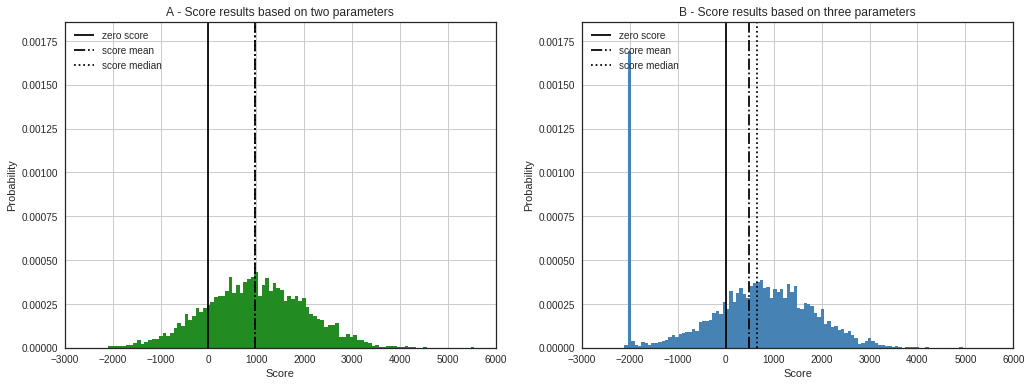
\includegraphics[width=1\textwidth]{Figures/score_results1.png}
				\caption{Posterior probability distributions from modeling scores using two (A) and three parameters (B) (reservoir thickness, reservoir top depth and seal thickness with a safety threshold of 20~m).}\label{fig:score_results1}
			\end{figure}
			Results from scoring based on simple Monte Carlo error propagation using only the priors of the 1D model (as defined in Section \ref{sec:1D_construction}) are plotted in Figure \ref{fig:score_results1}. A test run of scoring with only the two parameters reservoir thickness and depth, is shown in Figure \ref{fig:score_results1} (A). These results are represented by an approximately normal distribution. The score is negative in about 17\% of the cases. Mean and median are about the same.\\	
			Full scoring results, including also seal reliability (with a threshold of 20~m) as a parameter, are visualized in Figure \ref{fig:score_results1} (B). The main distribution is not changed significantly, except for a striking peak of probability at the possibility for a score of -2000. This presumably represents the bulk of cases, in which the seal is assumed to have failed. Regarding this, it is to be noted, that the mean of the seal top distribution is found at -2000 m. It can be seen in Figure \ref{fig:update_moderate1} (A1), that around that depth in the model column, reservoir top and seal top probability distributions significantly overlap. Thus, there is a possibility for a higher score, due to a shallower reservoir top position, but also a high probability for a seal thickness below the safety cut-off threshold of 20~m. The negative score peak at -2000 is thus presumably caused by a high number of seal failures, due to both layer interfaces located within this range. Furthermore, as a consequence of this negative peak, mean and median of the score distribution have been shifted to lower values and are now found further apart (see Figure \ref{fig:score_results1} (B)).\\
			Using this prior score distribution as a base, the custom loss function including risk was applied (see Figure \ref{fig:1D_LFR}). It can be observed that the minima for expected loss, i.e. the Bayesian estimators for differently risk-affine actors, are located at different estimates. Mean and median of the score distribution are clearly surpassed by the best estimate of the most risk-friendly actor (\textit{r} = 0.5), while for the most risk-averse actors (\textit{r} = 1.25 and \textit{r} = 1.5), the Bayes action equals a zero score estimate and thus the decision to take no action. It can also be recognized that the expected loss is generally lower for risk-friendlier actors on the side of positive estimates, which in this case is the relevant side for decision-making.		
			%\subsection{Applying the custom loss function on the 1D reservoir scores}
			%\begin{figure}[p!]
			%	\centering
			%	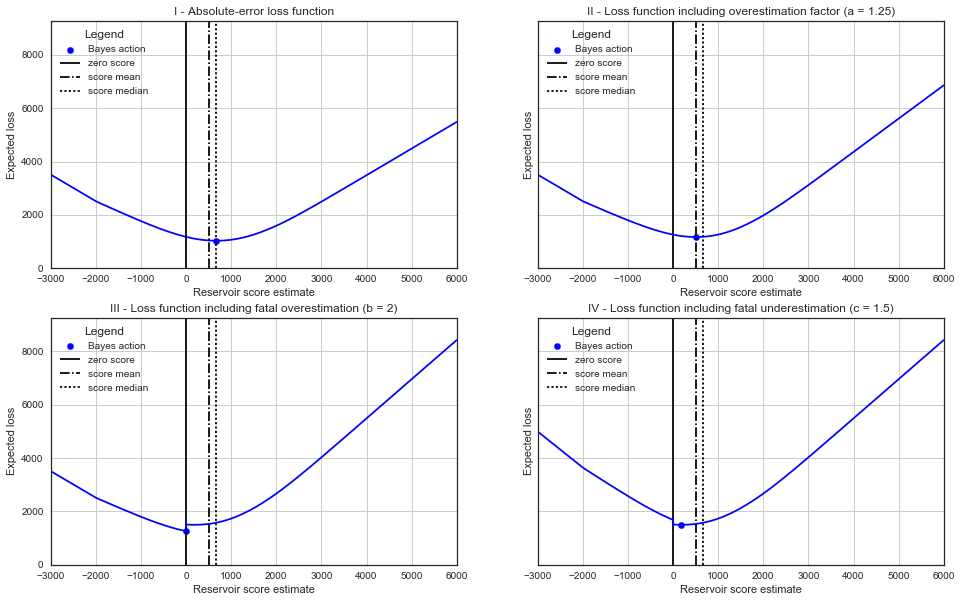
\includegraphics[width=1\textwidth]{Figures/LF_4steps.png}
			%	\caption{The single steps of customizing the loss function are depicted in plots I to IV.}\label{fig:LF_4steps}
			%\end{figure}			
			\begin{figure}[h]
				\centering
				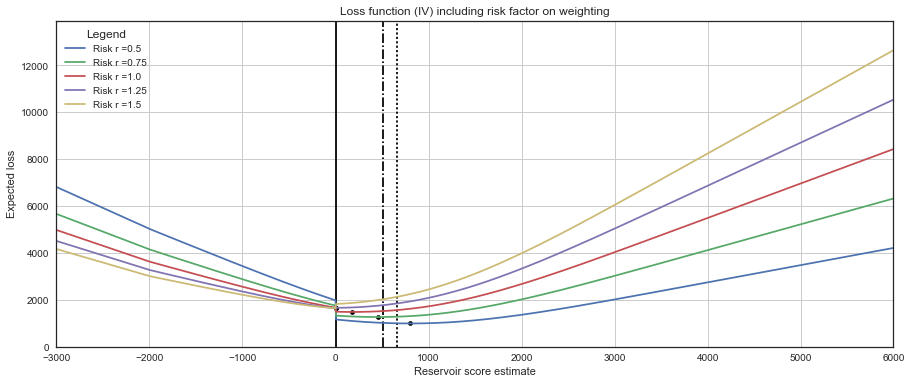
\includegraphics[width=1\textwidth]{Figures/LFR.png}
				\caption{Plotting of expected loss realizations after including the risk factor $r$ in the loss function  for actors with risk-affinities ranging from risk-averse ($r$ = 0.5 and 0.75), over risk-neutral ($r$ = 1), to risk-friendly ($r$ = 1.25 and $r$ = 1.5), based on the application of the custom loss function (Equation \ref{eq:LFR_final}) on a prior score distribution (see Figure \ref{fig:score_results1} (B)) from simple Monte Carlo error propagation.}\label{fig:1D_LFR} 
			\end{figure}			
			%Realizations of the four loss function adaption steps as elaborated in Section \ref{sec:LF_design} and based on the scoring results shown in Figure \ref{fig:score_results1}-B are depicted in the plots in Figure \ref{fig:LF_4steps}.
			%As expected, the median is returned for the Bayes action, when using the standard symmetric absolute-error loss function (Figure \ref{fig:LF_4steps}-I). Compared to this, it can be observed that assigning a stronger weight on overestimation (Figure \ref{fig:LF_4steps}-II) steepens the curve on the right hand side and shifts the minimum to the left, i.e. to a lower estimate. Using \textit{a} = 1.25, the Bayes action changes from the median, to a value close to the mean of the distribution. The shift and steepening are significantly reinforced by the introduction of fatal overestimation (Figure \ref{fig:LF_4steps}-III). With \textit{b} = 2, the Bayes action drops to the zero score estimate. It can also be noted, that by defining a condition dependent on the algebraic sign of the values, according to which only losses for positive estimates are multiplied by \textit{b}, a distinct jump appears at the zero score boundary. Due to a similar condition, the same effect is observed on the negative side of estimate values, where the curve has also been steepened, after including fatal underestimation (Figure \ref{fig:LF_4steps}-IV). This comes with a shift of the minimum towards positive values. It is also to be noted that with every customization step, the overall expected loss is increased.\\			
			%The implementation of the final custom loss function (Figure \ref{fig:LF_4steps}-IV) using single determined values for the true score is plotted in Figure \ref{fig:LF4_det_values}. This helps to clarify the way real losses result for each guess, relative to given true score values. The expected loss is acquired by arithmetically averaging such loss realizations based on the true score probability distribution by using Equation \ref{eq:ExpectedLoss2}.\\			
			%Implementing risk-affinity as a factor \textit{r} leads to different steepnesses of the plotted curves depicting loss and expected loss. The effect on the latter is visualized in Figure \ref{fig:1D_LFR}, where 0.5, 0.75, 1, 1.25 and 1.5 were chosen as values for \textit{r}. 

			\subsection{Bayesian inference using thickness likelihoods}	
			\begin{figure}[p!]
				\centering
				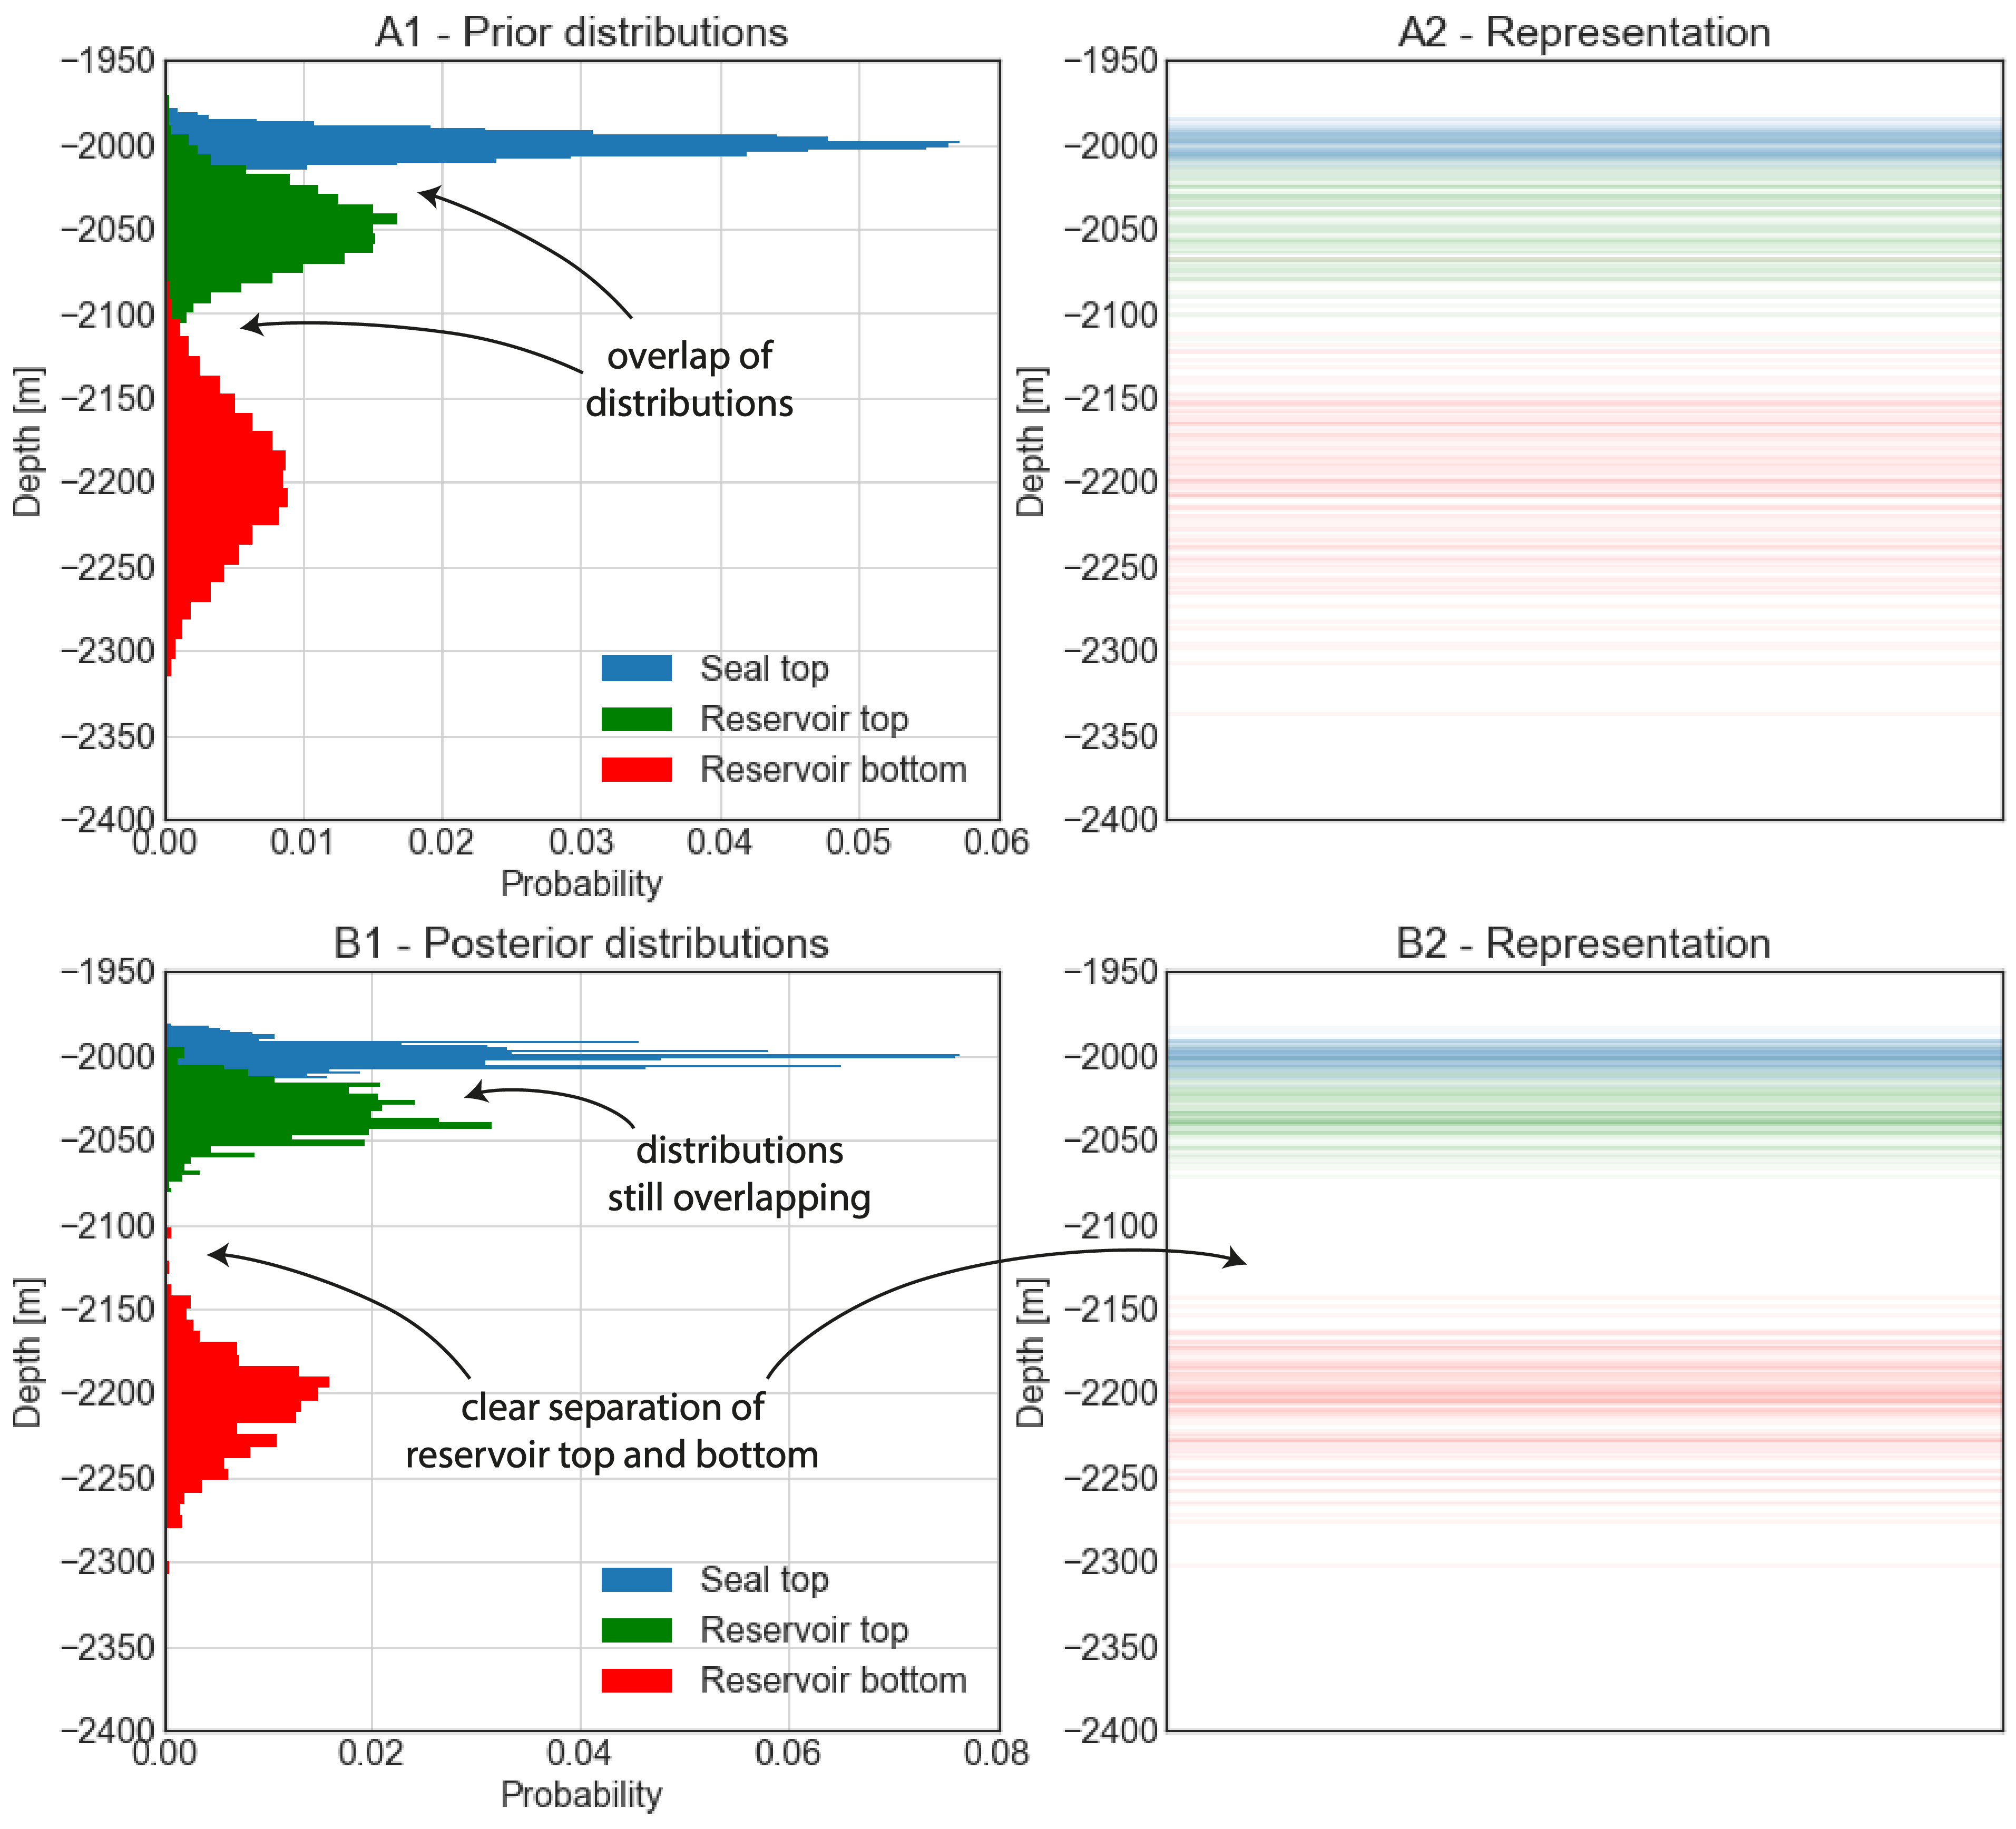
\includegraphics[width=1\textwidth]{Figures/update_moderate1.png}
				\caption{Prior (A1) and posterior distributions (A2) of the layer boundary positions in depth and respective representations (A2, B2). Bayesian inference was conducted using likelihoods defined as follows: Seal thickness: $\mu = 25~m; \sigma = 20~m$; reservoir thickness: $\mu = 180~m; \sigma = 40~m$. From (A1) to (B1), the distributions are slightly narrowed. Seal top and reservoir top distributions are still overlapping in (B1). A moderate reduction in uncertainty is also indicated by the representation in (B2), compared to (A2).}\label{fig:update_moderate1} 
			\end{figure}
			%\citet{delaVarga2016} made use of Bayesian inference to reduce the uncertainty in this type of one-dimensional model. The same was conducted here, as shown in the following.The locations of the layer boundaries are treated as priors with respective probability distributions. Now it is assumed that new observations have been made, providing additional information on the likelihoods of the thicknesses of the two layers. Likelihood functions for reservoir and seal thicknesses are introduced in the form of normal distributions, defined by means and standard deviations. These parameters vary according to nature of the observations made. Using the principle of Bayesian inference as explained in Chapter \ref{sec:bayes}, the model is updated and new posterior distributions for our true reservoir score are attained.\\
			Three representative Bayesian updating cases based on different sets of likelihoods in the 1D model are presented in the following. In each case, the layer boundaries defined in Section \ref{sec:1D_construction} were adopted as prior parameters. The various results from modeling with likelihoods, i.e. applying Bayesian inference, are compared to the original results and evaluations based on simple Monte Carlo error propagation using only priors.
				
				\subsubsection{Inference case I: Moderately reinforcing or ambivalent information}
				\begin{figure}[h]
					\begin{subfigure}{1\textwidth}
						\centering
						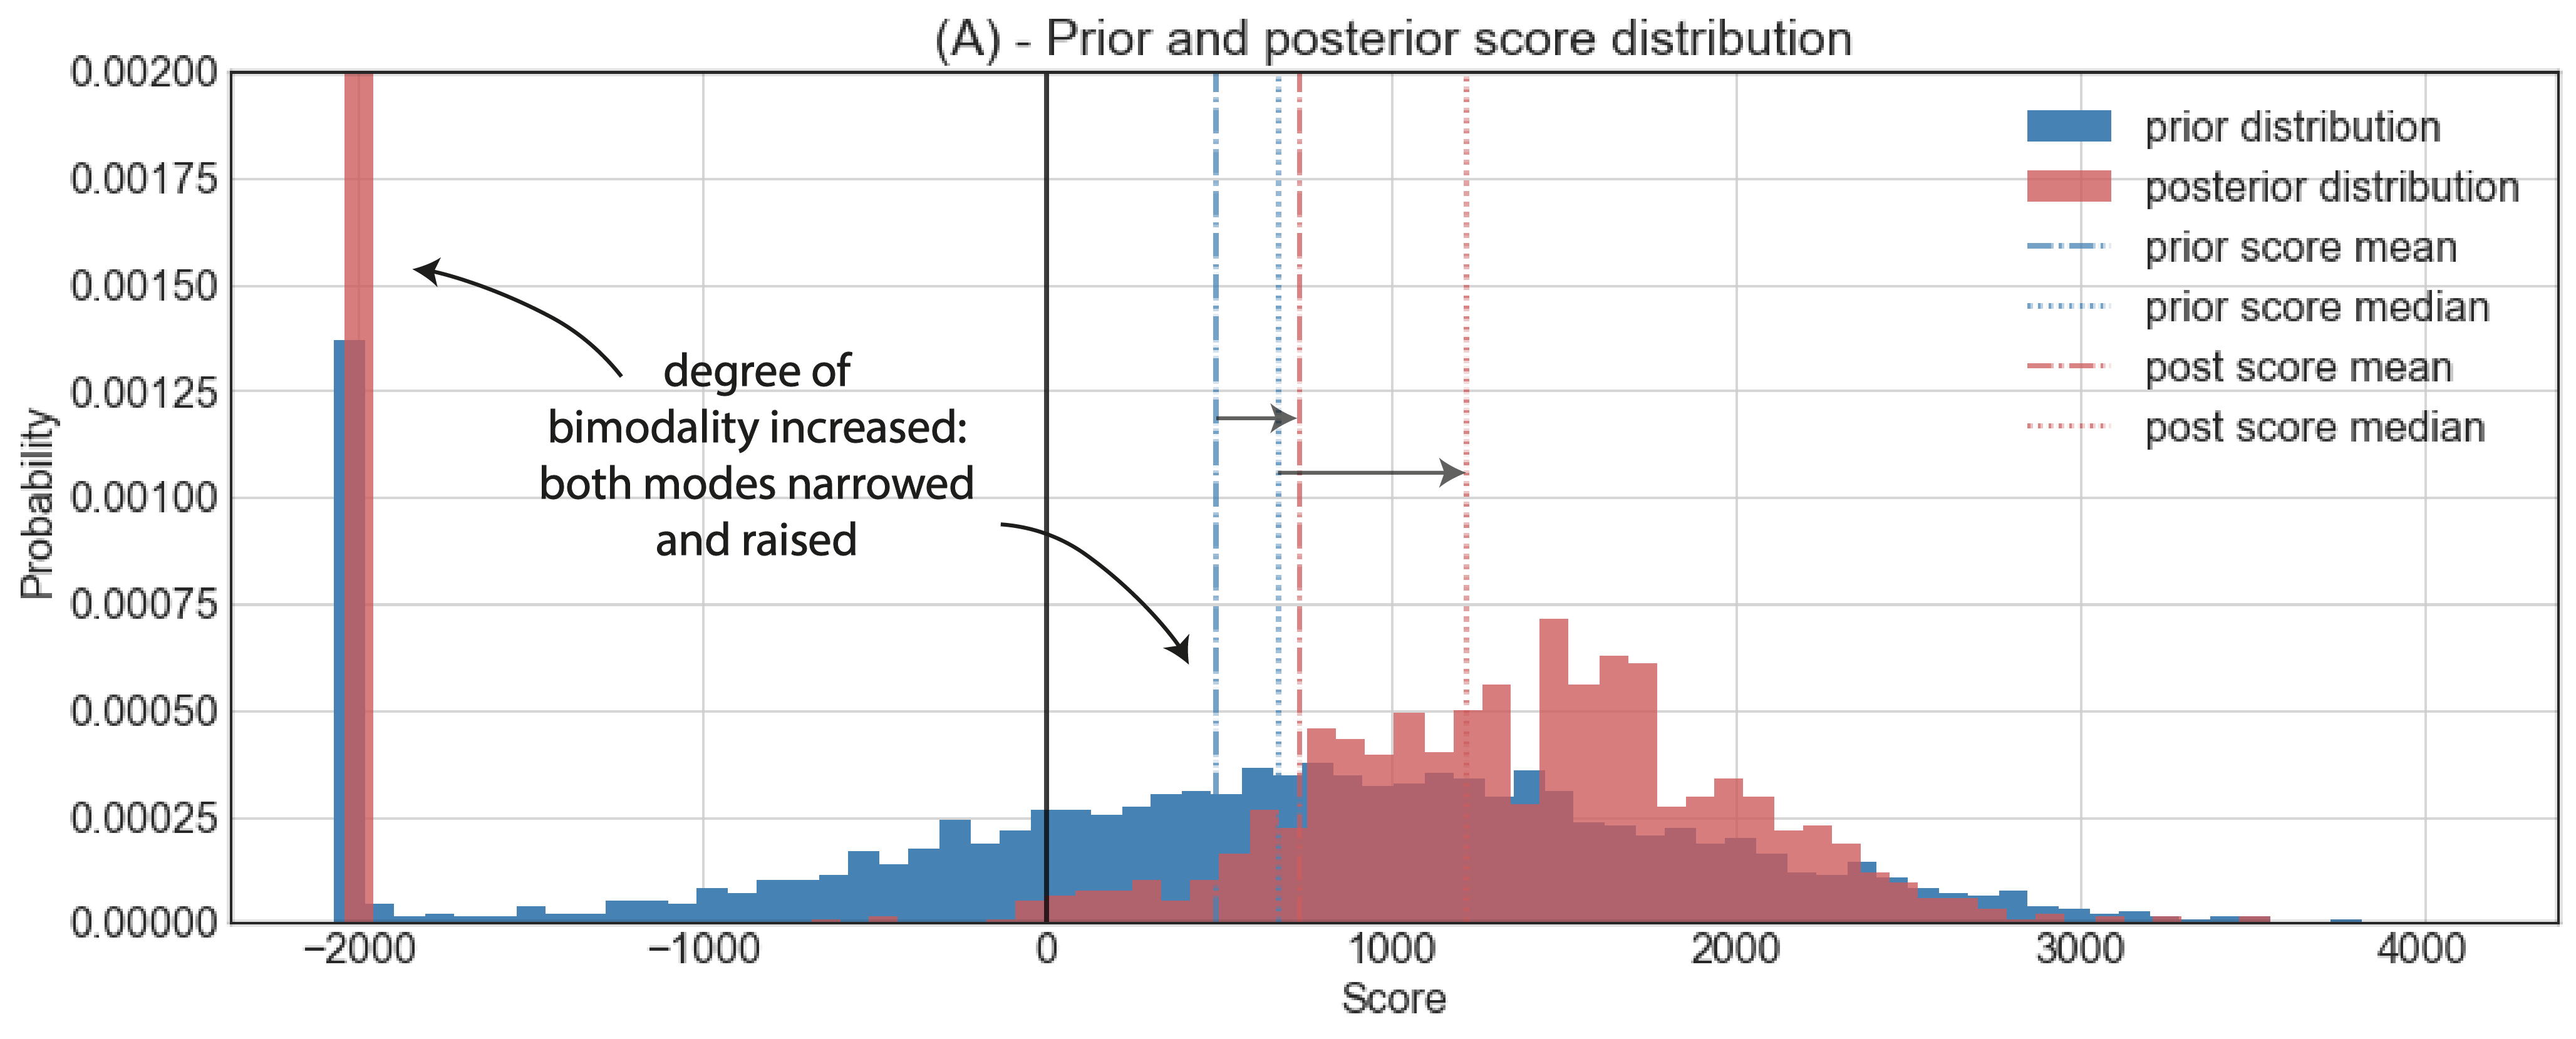
\includegraphics[width=1\linewidth]{Figures/update_moderate2.png}
						%\caption{1a}
						%\label{fig:sfig1}
					\end{subfigure}%
					\\
					\begin{subfigure}{1\textwidth}
						\centering
						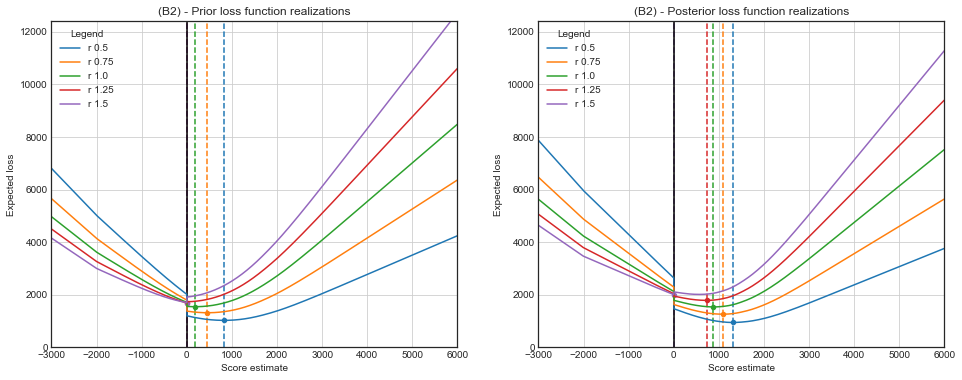
\includegraphics[width=1\linewidth]{Figures/update_moderate3.png}
						%\caption{1b}
						%\label{fig:sfig2}
					\end{subfigure}
					\caption{Reservoir score distributions (A) and change in the realizations of expected loss for several risk parameters (B1, B2) before and after Bayesian updating based on likelihoods defined as follows: Seal thickness: $\mu = 25~m; \sigma = 20~m$; reservoir thickness: $\mu = 180~m; \sigma = 40~m$.}
					\label{fig:update_moderate2_3}
				\end{figure}				
				In this first case, a normal distribution with a mean ($\mu$) of 25~m and a standard deviation ($\sigma$) of 20~m was chosen to reflect the likelihood of the seal thickness. For the reservoir, a normal distribution with a mean of 180~m and a standard deviation of 40~m was used respectively. As can be observed in Figure \ref{fig:update_moderate1}), the uncertainty in the probability distributions for the positions of layer boundaries in depth was reduced moderately, mostly for the reservoir bottom, by conducting Bayesian inference with these values.\\					
				Scoring was applied based on these new distributions. In Figure \ref{fig:update_moderate2_3} (A), it can be recognized that the bulk of the score distribution was shifted to the positive side of values and narrowed, approximately resembling a normal distribution there. However, the peak at -2000 was raised, while the probability of scores between -2000 and 0 was decreased to be negligible, i.e. the true score is most likely either positive or -2000, if it is negative. So while uncertainties were reduced in areas of opposite sign, the divide between these was significantly increased. The overall uncertainty seems thus to have been widely maintained and barely transformed into a problem of duality. The change in uncertainty might thus me described as ambivalent.\\
				Application of the custom loss function (Equation \ref{eq:LFR_final}) is visualized in Figure \ref{fig:update_moderate2_3}, in which the expected losses are compared before (B1) and after (B2) Bayesian inference. It is observable, that by adding information about layer thickness likelihoods, Bayes actions were shifted relative to the nature of the information. In this case, the added data generally reinforces the probability of the reservoir to be sufficiently thick. Information on the seal, however, based on a normal distribution around 25~m thickness, leaves high uncertainty about the reliability of the seal, as the safety threshold is defined as 20~m. Consequently, the risk of complete seal failure remains a major concern.\\				
				Increased certainty about the reservoir thickness was sufficient to shift Bayes actions to higher estimates for all actors. Estimates of the more risk neutral actors ($r = 0.5$ to $r=1.25$) were increased the most. This has led to a slight convergence of the Bayes actions. Expected losses were altered only slighty. For the risk neutral actor, this change is negligible. For risk-friendlier actors, the expected loss was decreased, but for risk-averse actors, as they shifted from zero ("take no action") to positive estimates, increased.\\	
				%These shifts are quantified in Table \ref{tab:update_examples_all}.Expected losses are decreased for the risk-neutral and the two risk-friendlier individuals. It is clear that the expected loss was reduced the most for the risk-friendliest actor and it increased most significantly for the most risk-averse actor.
				%\begin{table}
				%	\centering
				%	\begin{tabular}[c]{| l | l | l |}
				%		\hline
				%		Risk factor \textit{r} & Shift in Bayes action & Change in expected loss \\ \hline
				%		0.50 & +~553.67 & -~105.49 \\ 
				%		0.75 & +~673.40 & -~81.67  \\ 
				%		1.00 & +~750.05 & -~33.56 \\ 
				%		1.25 & +~713.19 & +~75.71 \\ 
				%		1.50 & +~0.00 & +~282.64  \\ 
				%		\hline
				%	\end{tabular}
				%	\caption{Bla}
				%	\label{tab:update_moderate_tab}
				%\end{table}
								
				\subsubsection{Inference case II: Likely reliable seal}
				\begin{figure}[h]
					\begin{subfigure}{1\textwidth}
						\centering
						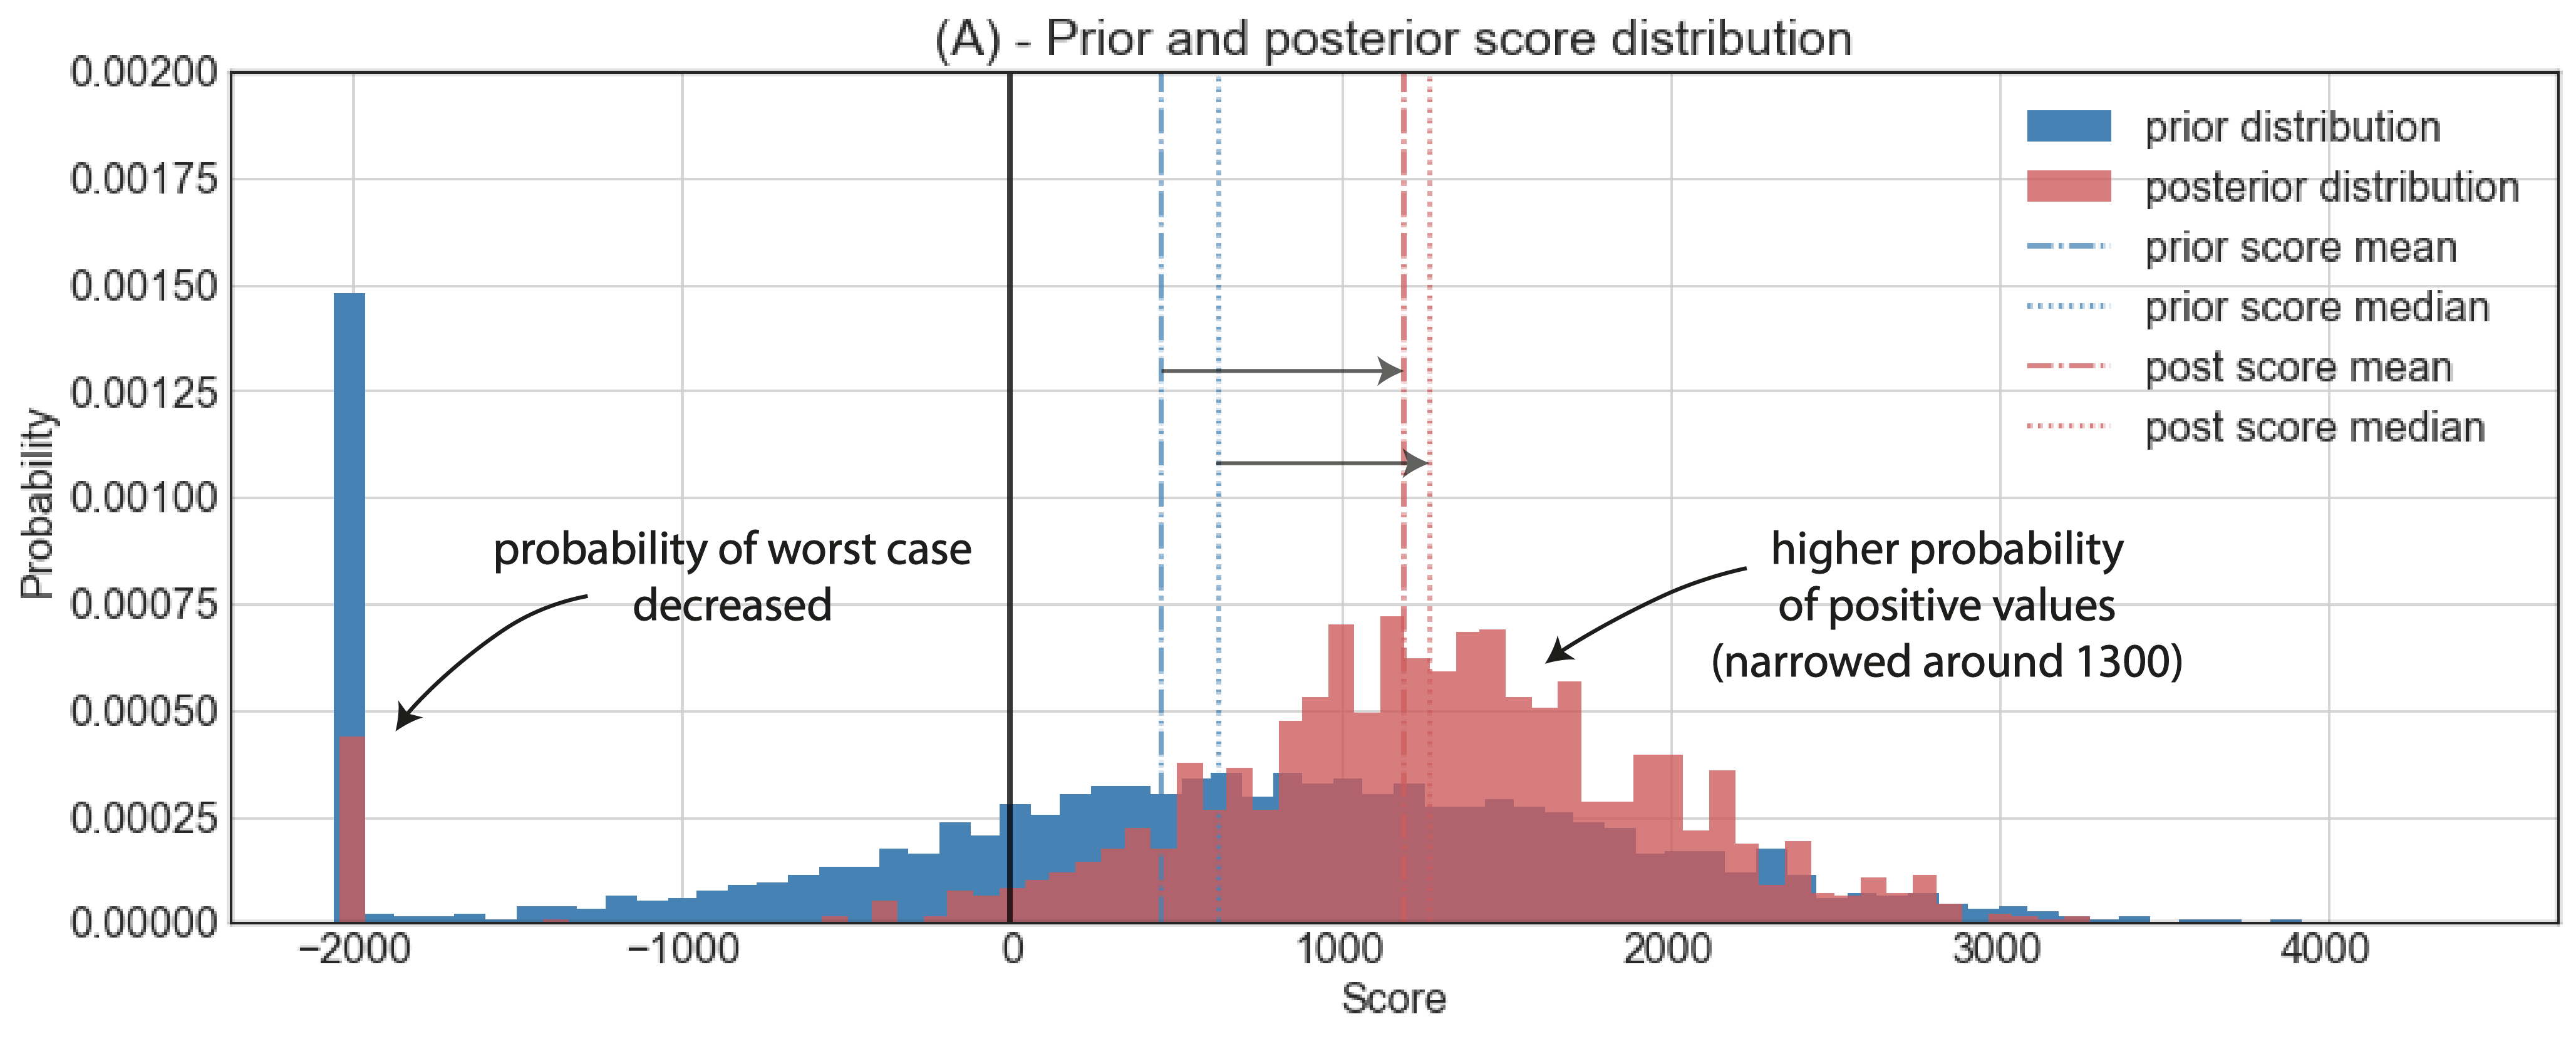
\includegraphics[width=1\linewidth]{Figures/update_goodseal2.png}
						%\caption{1a}
						%\label{fig:sfig1}
					\end{subfigure}%
					\\
					\begin{subfigure}{1\textwidth}
						\centering
						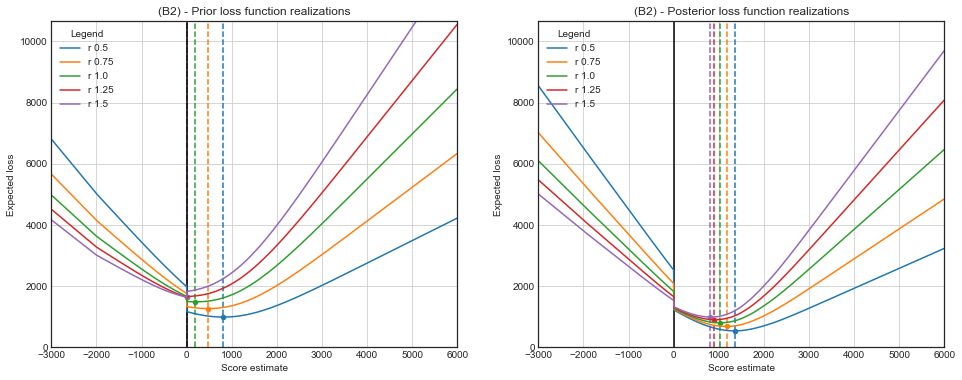
\includegraphics[width=1\linewidth]{Figures/update_goodseal3.png}
						%\caption{1b}
						%\label{fig:sfig2}
					\end{subfigure}
					\caption{Reservoir score distributions (A) and change in the realizations of expected loss for several risk parameters (B1, B2) before and after Bayesian updating based on likelihoods defined as follows: Seal thickness: $\mu = 50~m; \sigma = 20~m$; reservoir thickness: $\mu = 180~m; \sigma = 40~m$.}
					\label{fig:update_goodseal2_3}
				\end{figure}
				In this second case, the reservoir thickness likelihood was defined in the same way as in case I ($\mu = 180~m; \sigma = 40~m$). For the seal, a higher mean of 50~m with a standard deviation of 20~m was chosen, favoring the likelihood of a reliable seal relative to the threshold of 20~m thickness. Respective score results are depicted in Figure \ref{fig:update_goodseal2_3} (A). The bulk of the distribution is narrowed on the positive side of estimates. Very apparent is the significant diminishment of the "seal failure peak" at -2000. Due to this, in combination with the overall distribution narrowing, mean and median were clearly shifted to higher values and are now much closer together.\\	
				Applying the custom loss function on this new score distribution resulted in the realizations of expected loss illustrated in Figure \ref{fig:update_goodseal2_3}. Bayes actions were shifted clearly to higher estimates and expected losses of these minima were significantly reduced for all actors. The risk-neutral to risk-averse individuals seem to have profited the most, due to a large change in estimate value and decreased expected loss. Compared to the foregone case, a higher degree of overall uncertainty reduction was achieved. The risk of seal failure is now much lower. Consequently, Bayes actions were not only shifted to greater values, but also narrowed significantly in their range, i.e. the optimal decisions of the different actors have converged to a much greater extent than in case I.\\		
				%This is quantified in Table \ref{tab:update_examples_all}. According to these values,  Compared to case I, the estimate shifts for both risk-friendlier actors remain approximately the same, expected losses, however, are lowered much more significantly.
				%\begin{table}
				%	\centering
				%	\begin{tabular}[c]{| l | l | l |}
				%		\hline
				%		Risk factor \textit{r} & Shift in Bayes action & Change in expected loss \\ \hline
				%		0.50 & +~522.95 & -~436.26 \\ 
				%		0.75 & +~697.73 & -~551.92  \\ 
				%		1.00 & +~855.57 & -~631.92 \\ 
				%		1.25 & +~912.43 & -~647.10 \\ 
				%		1.50 & +~819.26 & -~545.96  \\ 
				%		\hline
				%	\end{tabular}
				%	\caption{Bla}
				%	\label{tab:update_goodseal_tab}
				%\end{table}
				
				\subsubsection{Inference case III: Safe seal but likely subpar reservoir thickness}
				\begin{figure}[h]
					\begin{subfigure}{1\textwidth}
						\centering
						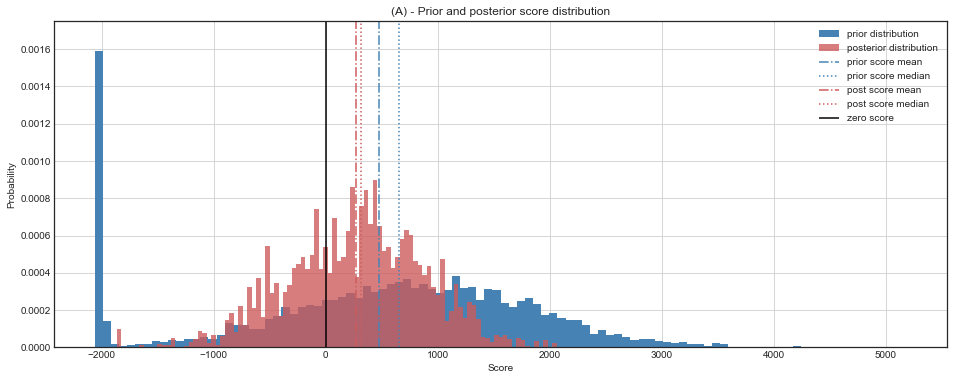
\includegraphics[width=1\linewidth]{Figures/update_smallres2.png}
						%\caption{1a}
						%\label{fig:sfig1}
					\end{subfigure}%
					\\
					\begin{subfigure}{1\textwidth}
						\centering
						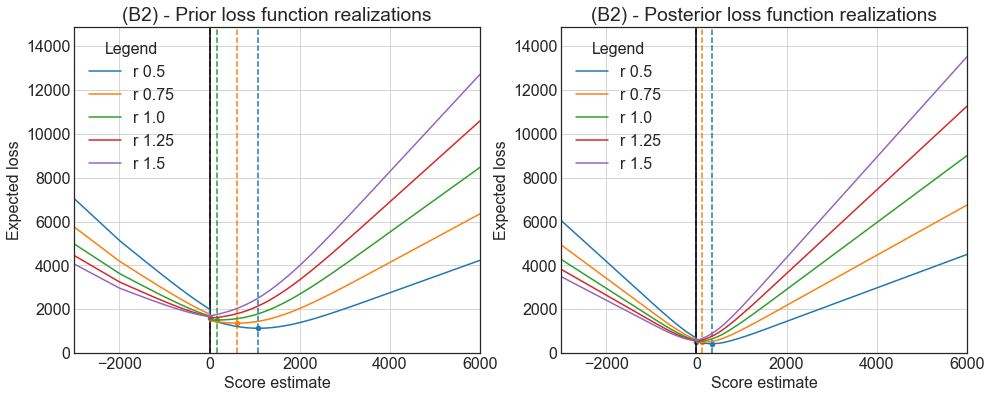
\includegraphics[width=1\linewidth]{Figures/update_smallres3.png}
						%\caption{1b}
						%\label{fig:sfig2}
					\end{subfigure}
					\caption{Reservoir score distributions (A) and change in the realizations of expected loss for several risk parameters (B1, B2) before and after Bayesian updating based on likelihoods defined as follows: Seal thickness: $\mu = 70~m; \sigma = 10~m$; reservoir thickness: $\mu = 100~m; \sigma = 30~m$.}
					\label{fig:update_smallres2_3}
				\end{figure}
				In this third case, seal safety was ensured by using a mean of 70~m with a standard deviation of 10~m for the seal thickness likelihood. However, the new observations were assumed to provide information about the reservoir unit that makes it likely to be thinner than expected. Reservoir thickness likelihood was assigned a mean of 100~m and a standard deviation of 30~m.\\
				The subsequent score distribution is depicted in Figure \ref{fig:update_smallres2_3} (A). It can be seen that while the whole distribution was strongly narrowed, it also was shifted to the left, to lower and negative estimates. Mean and median are almost equal, indicating narrowing towards symmetry in the shape of a normal distribution. As seal reliability is practically guaranteed, the peak at -2000 has vanished.\\				
				Based on this posterior score probability distribution, Bayes actions were shifted to lower estimates for all actors using the custom loss function (see Figure \ref{fig:update_smallres2_3} (B2)). The risk-neutral and both risk-averse individuals find their Bayesian estimators to be zero after updating, i.e. bidding on a positive score is deemed to be too risky to them. There is no shift in estimate for risk-averse actors, as they already found their best estimates to be zero before updating. Notable is the large reduction of expected loss in general. The range of Bayes actions was significantly narrowed. Overall, it is apparent that uncertainty was significantly reduced (see the narrowed distribution). However, although the seal can expected to be safe, the reservoir thickness is likely subpar. Due to this, the distribution was shifted to lower and negative values, strongly increasing the probability of an unfavorable true score. Consequently, only risk-friendly actors are willing to take action.
				%Quantified changes in the positions and values of the Bayes actions are listed in Table \ref{tab:update_examples_all}. Furthermore, the spread of expected loss values around the minima for all actors was diminished. In other words, the expected loss values of the Bayes actions are now much closer to each other.
				%\begin{table}
				%	\centering
				%	\begin{tabular}[c]{| l | l | l |}
				%		\hline
				%		Risk factor \textit{r} & Shift in Bayes action & Change in expected loss \\ \hline
				%		0.50 & -~498.98 & -~538.08 \\ 
				%		0.75 & -~346.16 & -~717.83  \\ 
				%		1.00 & -~176.13 & -~872.02 \\ 
				%		1.25 & -~0.00 & -~946.04 \\ 
				%		1.50 & -~0.00 & -~951.57  \\ 
				%		\hline
				%	\end{tabular}
				%	\caption{Bla}
				%	\label{tab:update_smallres_tab}
				%\end{table}
				% % % %
				% % % %
				%\begin{table}
				%	\centering
				%	\begin{tabular}[c]{| c || l | l || l | l || l | l |}
				%		\hline
				%		& Example I & & Example II & & Example III & \\
				%		\hline
				%		\hline
				%		\textit{r} & $\Delta$ BA & $\Delta$ EL & $\Delta$ BA & $\Delta$ EL & $\Delta$ BA & $\Delta$ EL\\ 
				%		\hline
				%		0.50 & +~553.67 & -~105.49 & +~522.95 & -~436.26 & -~498.98 & -~538.08 \\ 
				%		0.75 & +~673.40 & -~81.67 & +~697.73 & -~551.92 & -~346.16 & -~717.83  \\ 
				%		1.00 & +~750.05 & -~33.56 & +~855.57 & -~631.92 & -~176.13 & -~872.02 \\ 
				%		1.25 & +~713.19 & +~75.71 & +~912.43 & -~647.10 & -~0.00 & -~946.04 \\ 
				%		1.50 & +~0.00 & +~282.64 & +~819.26 & -~545.96 & -~0.00 & -~951.57  \\ 
				%		\hline
				%	\end{tabular}
				%	\caption{Changes in Bayes action (BA) and minimal expected loss (EL) for Bayesian updating cases I, II and III and respective actors with risk parameters $r$.}
				%	\label{tab:update_examples_all}
				%\end{table}
				% % % %
				% % % %
				%\begin{table}
				%		\begin{tabular}[c]{| l | l | l |}
				%			\hline
				%			Risk factor \textit{r} & Shift in Bayes action & Change in expected loss \\ \hline
				%			0.50 & -~498.98 & -~538.08 \\ 
				%			0.75 & -~346.16 & -~717.83  \\ 
				%			1.00 & -~176.13 & -~872.02 \\ 
				%			1.25 & -~0.00 & -~946.04 \\ 
				%			1.50 & -~0.00 & -~951.57  \\ 
				%			\hline
				%		\end{tabular}
				%		\caption{Bla}
				%		\label{tab:update_examples_all}
				%\end{table}
				
			%\subsection{General 1D model inference results}
			%This conceptual application in an abstract 1D geological model already serves to illuminate some of the main effects of Bayesian inference on decision-making. Three main mechanisms were observable in these cases: 
			%\begin{enumerate}
			%	\item \textbf{Lateral shifting} of the score distribution and consequent shift in Bayes actions along the axis of possible score estimates, while their expected losses remain approximately constant. To a certain degree, this seems to be independent from the overall uncertainty reduction and is primarily related to the shift of probability to a different area. According to this observation, uncertainty reduction is not a necessary condition to significantly alter the decisions for all individuals. 
				%An incentive to bid on higher estimates is given solely by the shift of the posterior distribution to higher values, while the inherited degree of uncertainty may remain the same.
			%	\item \textbf{Narrowing} of the score probability distribution, due to uncertainty reduction and consequent convergence of the Bayes actions of different actor's towards a similar estimate. Additionally, expected loss seem to decrease with uncertainty. If perfect information about our parameters was available, all individuals would bid on the same estimate and expected a loss of zero. 
			%	\item \textbf{Dualization} of uncertainty, apparently due to reduction of uncertainty that narrows probability to areas of two possible outcomes, such as success and failure. The area at which uncertainty is reduced seems to be of significance. A high reduction of uncertainty in the form of standard deviation near a cut-off threshold value seems to lead to a transformation of the nature of uncertainty to a problem of duality. CONNECTION TO SHIFTING???
			%\end{enumerate}
			%The second mechanism, i.e. uncertainty reduction, can thus presumed to be most significant regarding the process of "good" decision-making, as actor's wish to minimize their expected loss from bidding on an estimate. In an optimal case, this would come in combination with a shift of probabilities (first mechanism) to more positive values, so that a higher economic value may be returned from the acquisition of information.
			%As can be expected intuitively, reassurance of positive scores, for example by narrowing of the distribution of scores on the side of positive estimates or by reducing the occurrence of negative extrema, leads to shifts towards higher Bayes action estimates for all actors. Conversely, actors are discouraged to expect gains when facing a higher probability of negative scores. Unsurprising is also the inverse behavior of risk-averse and risk-friendly individuals. However, it is most notable that a reduction of uncertainty in any case leads to a diminished spread of Bayes actions between all actors. In other words, given better information about the true value of the reservoir, different actors come to more similar decisions. Given perfect information, all actors would presumably choose the same estimate, which would equal the true score.
				
		\section{3D geological model results}
		- first: MC simulation of only prior uncertainty error propagation to generate a prior reference model
		- second: Bayesian inference using only thickness likelihoods
		- third: Bayesian inference including SSF likelihood
		- last test: BI using only SSF likelihood
		
		\subsection{Prior model}
		\begin{figure}[h]
			\centering
			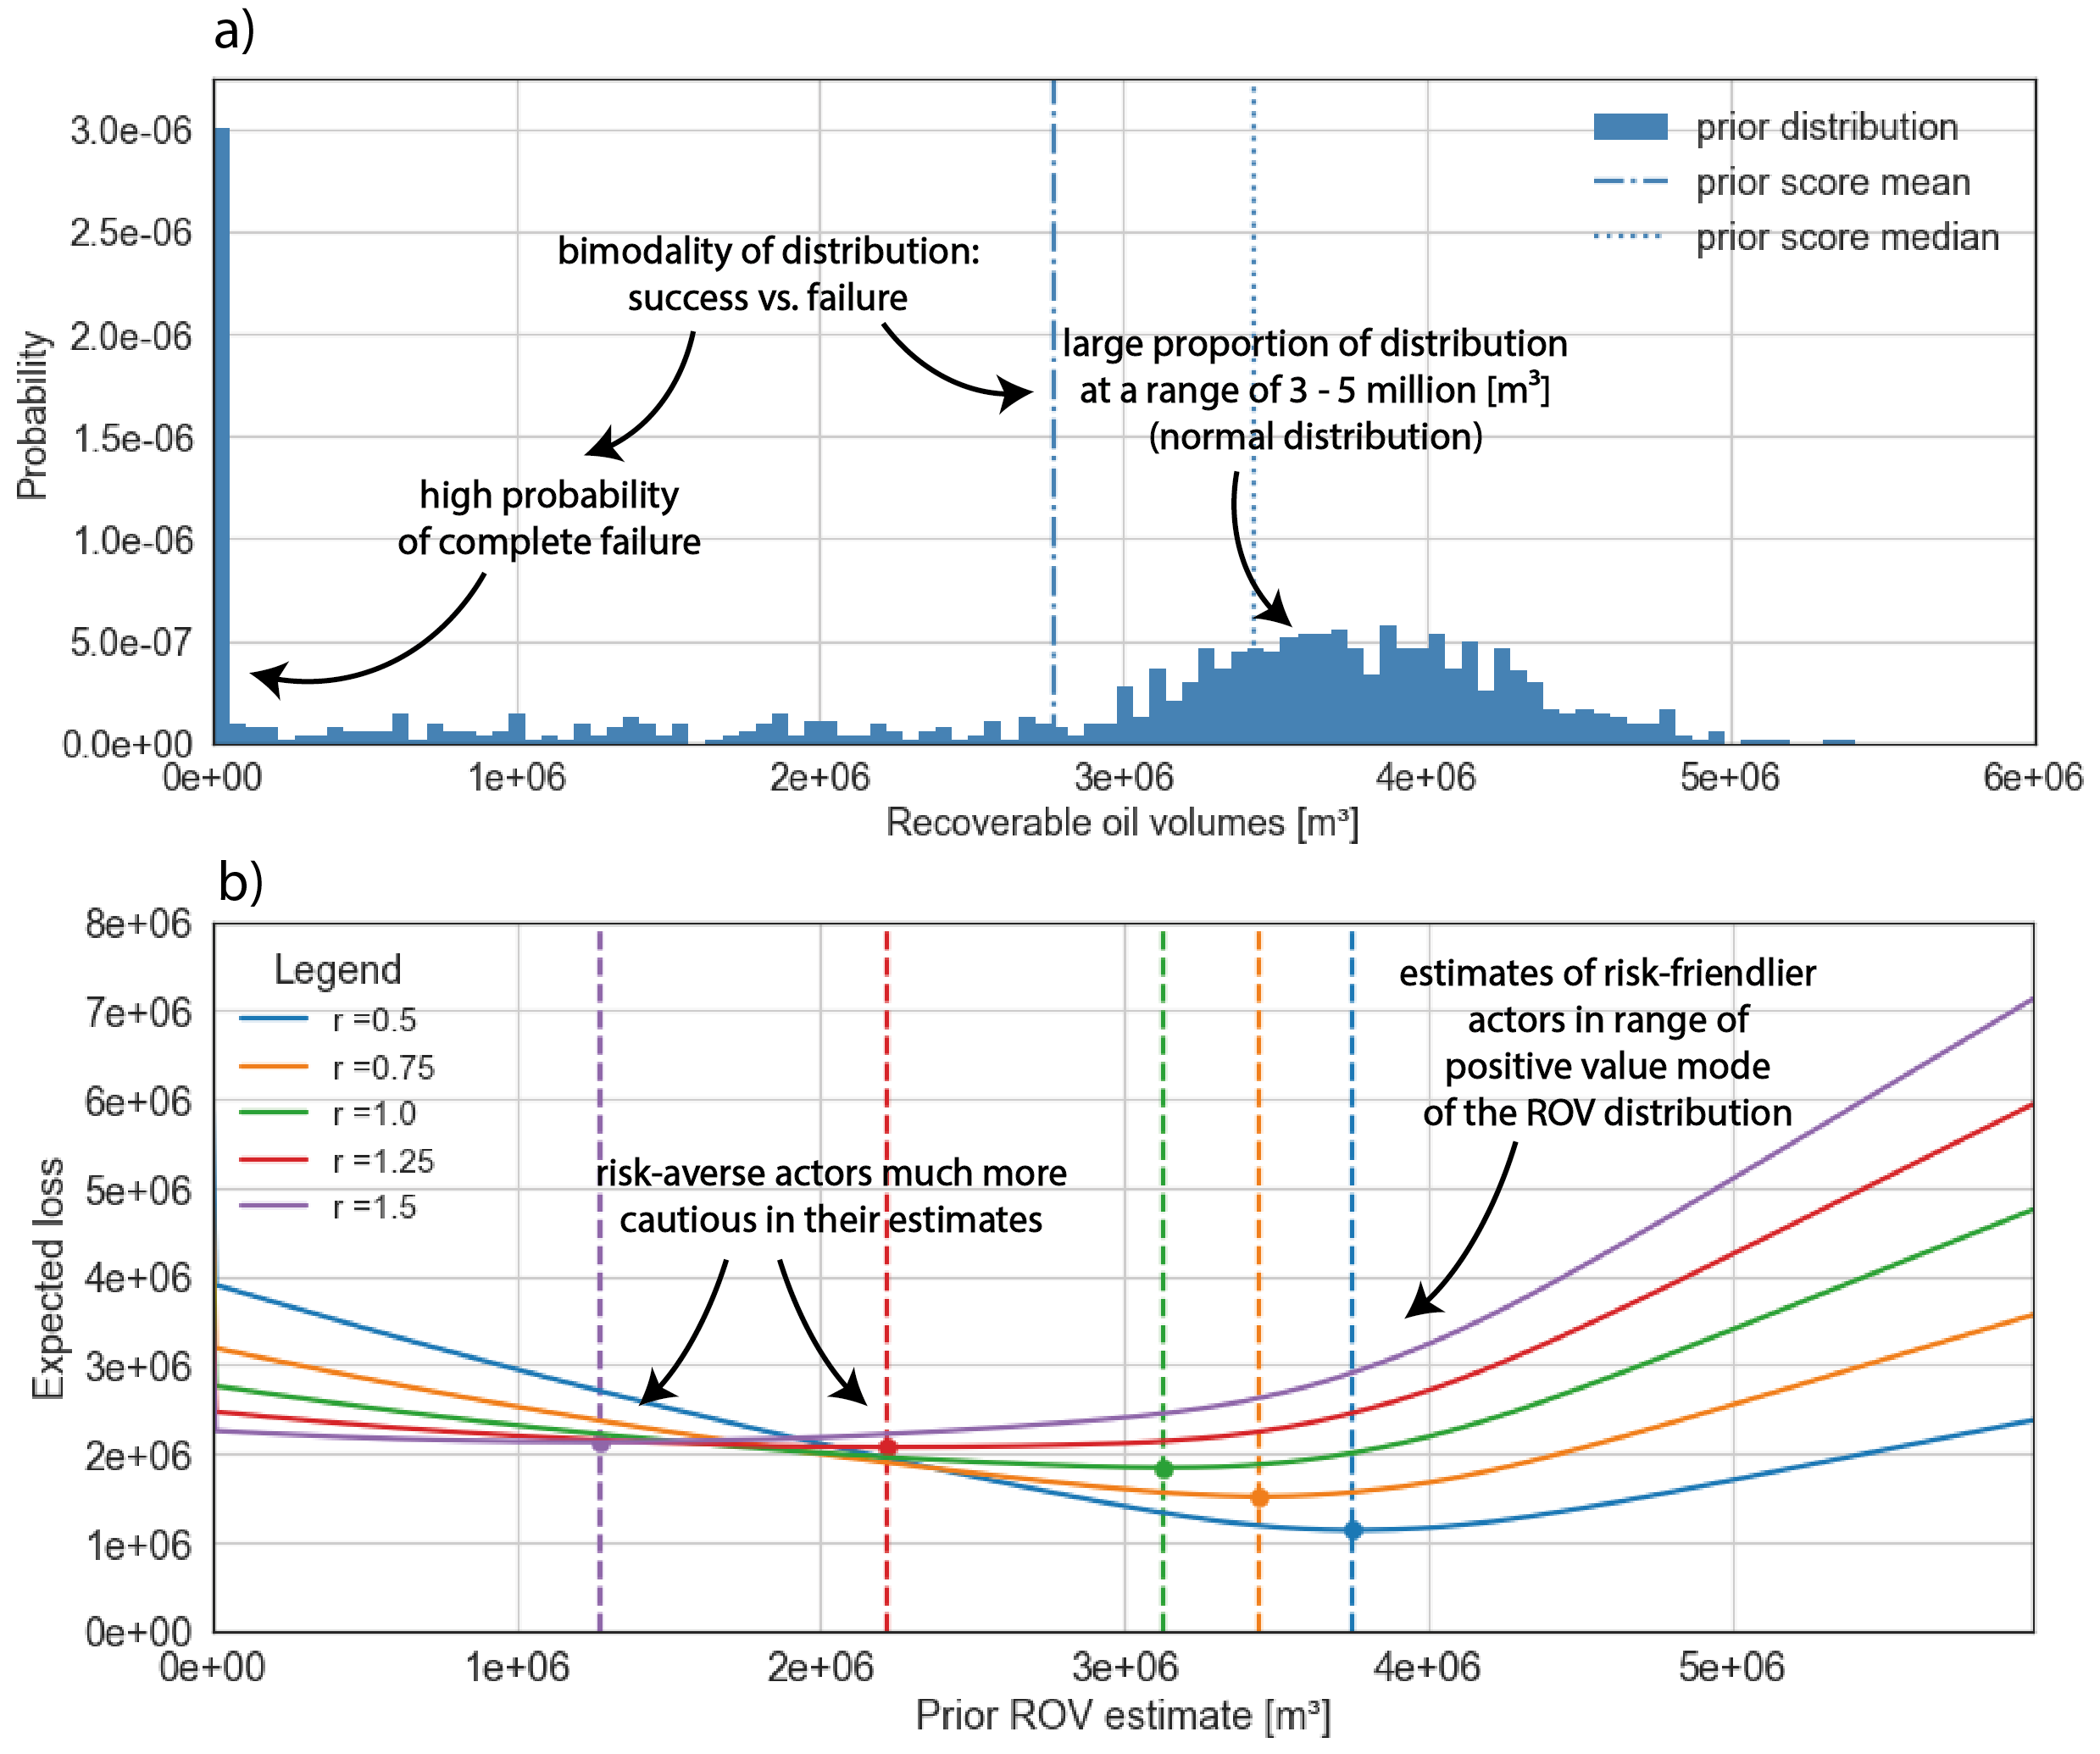
\includegraphics[width=1\textwidth]{Figures/M_prior}
			\caption{....}\label{fig:M_prior}
		\end{figure}
		
		\subsection{Posterior model I}
		\begin{figure}[p!]
			\centering
			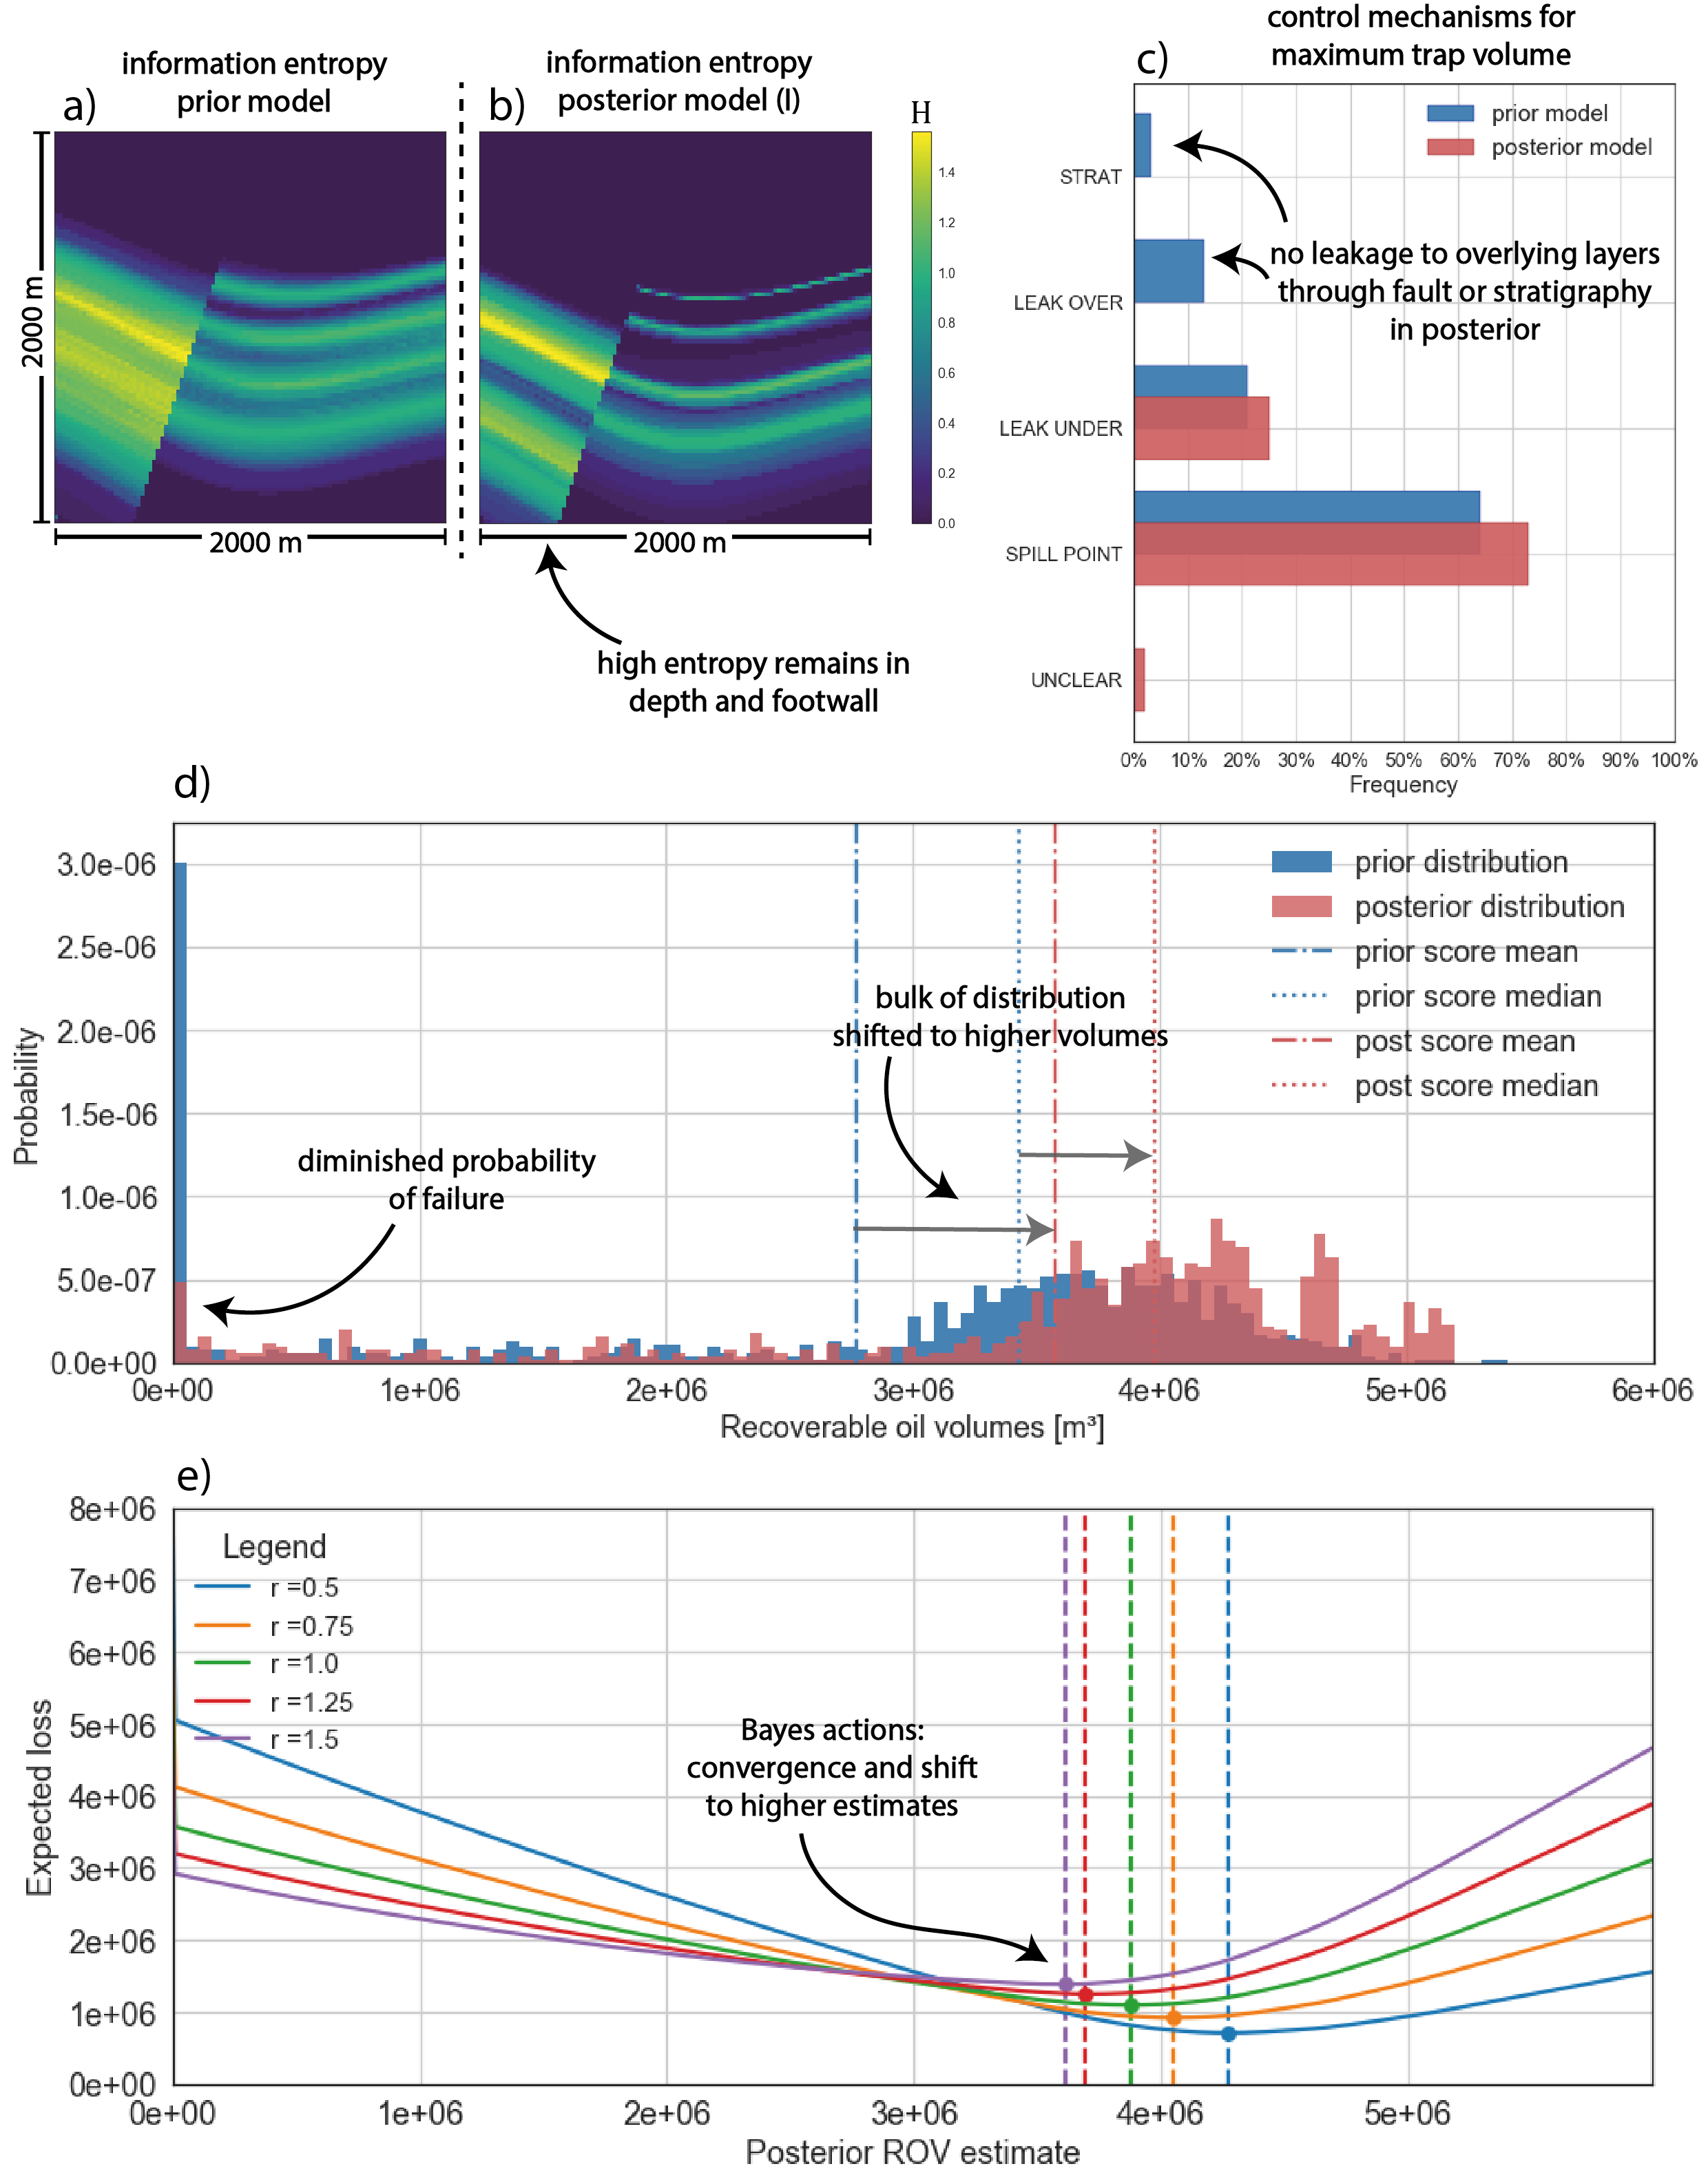
\includegraphics[width=1\textwidth]{Figures/ML1}
			\caption{....}\label{fig:ML1}
		\end{figure}
		
		\subsection{Posterior model II}%ML3
		-results similar to I, basically same
		- results of ML1 generally similar as for ML3:
		i.e. thicker reservoir does not mean higher volume, as we didn't implement a direct uncertainty to the shape, the spill point will stay more or less the same
		-> spill and leak point as limiting factors to max volume
		-> max volume already defined in prior (ROV max 5,500,000)
	
		\subsection{Posterior model III}%ML2
		\begin{figure}[p!]
			\centering
			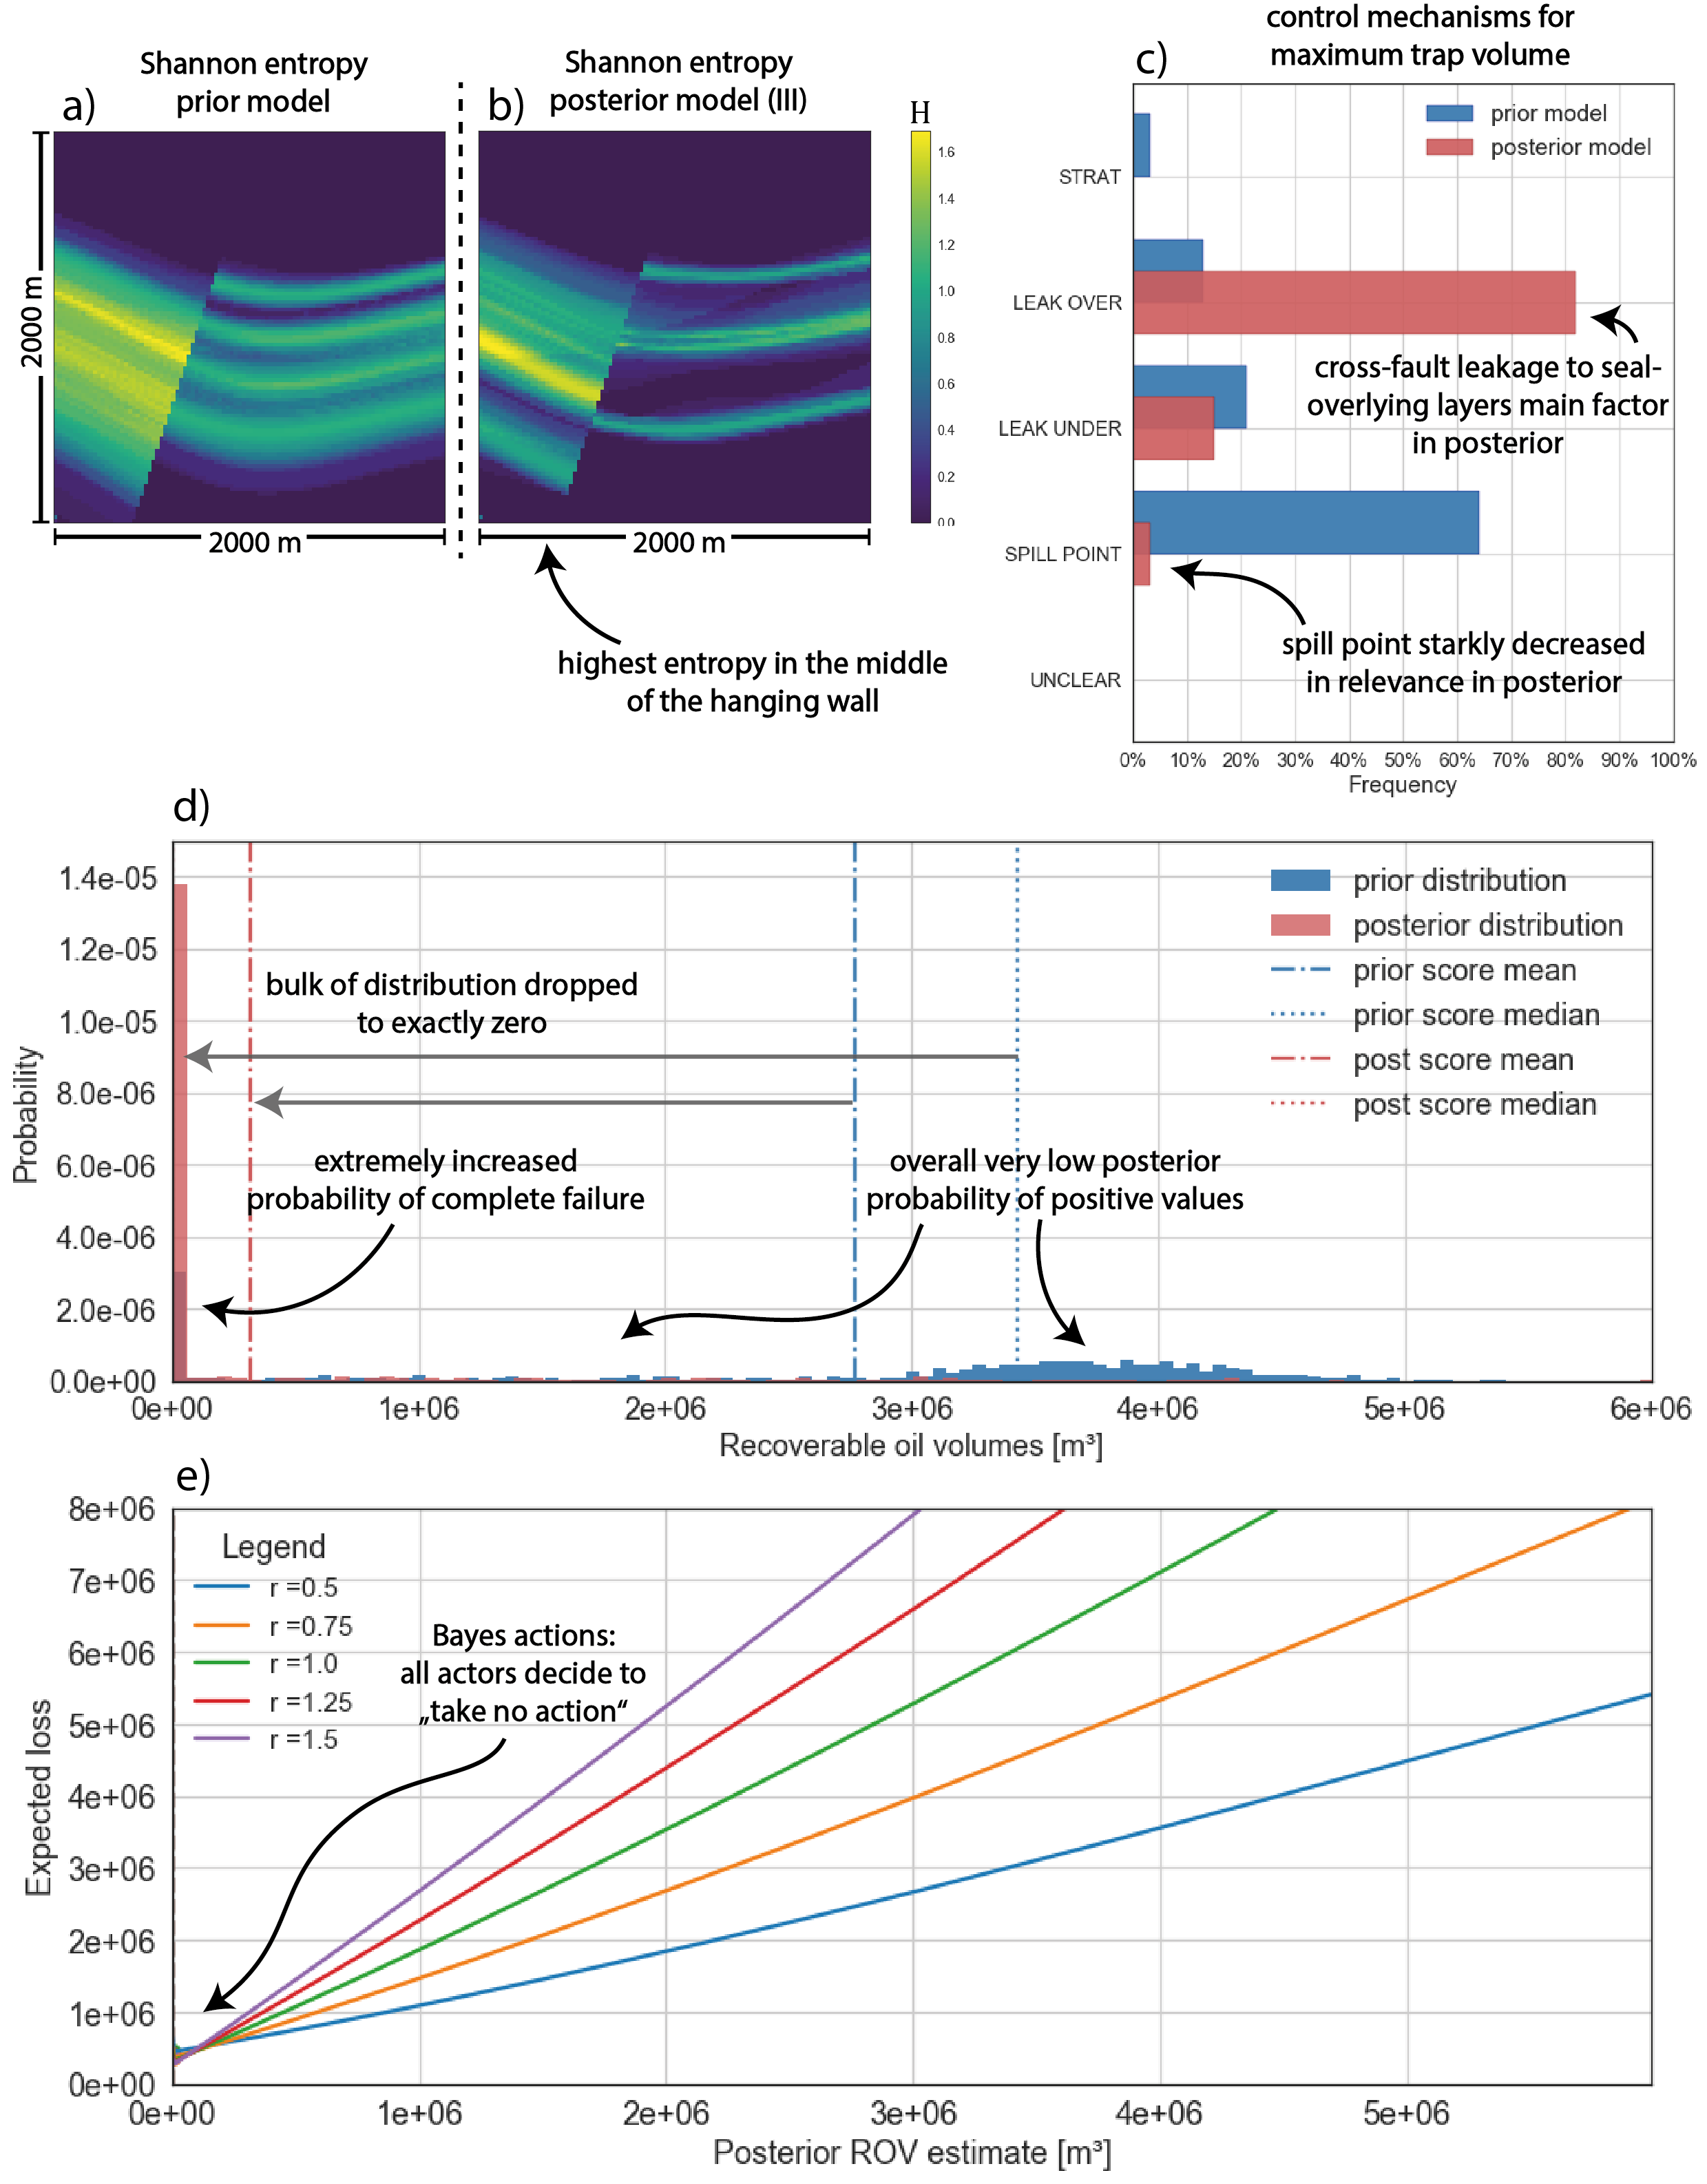
\includegraphics[width=1\textwidth]{Figures/ML2}
			\caption{....}\label{fig:ML2}
		\end{figure}
		- see ML2: seal thickness as decisive factor
			-> if seal thin and reservoir thick see the ratio of both!), higher likelihood of surpassing SSF
		